\documentclass[10pt,a4paper]{article}
\usepackage{graphicx}
\usepackage{amsmath}
\begin{document}
\begin{titlepage}
\begin{center}
\Large\textbf{Report DLP}\\
\large\textit{Bao,Viet}
\end{center}
\end{titlepage}
\section{Text2SQL}
\subsection{problem}
This task is to produce sql queries based on inputs consits of natural language question and database. The task can be formalized as: \\\\
Given a natural language $Q$ and the schema $S = \langle \mathcal{T},\mathcal{C}\rangle$ for a relational database, the parser needs to generate the corresponding SQL query $Y$. The schema consists of tables $\mathcal{T} = \{t_1,..,t_N\}$ and fields $\mathcal{C} =\{c_{11},...,c_{1|T_1|},...,c_{n1},...,c_{N|T_N|} \}$.Each table $t_i$ and each field $c_{ij}$ has a textual name. Some fields are primary keys, used for uniquely indexing each data record, and some are foreign keys, used to reference a primary key in a different table. In addition, each field has a data type, $\tau\in\{number,text,time,boolean,etc\}$.\\\\
 In the paper Bridging Textual and Tabular Data for Cross-Domain Text-to-SQL Semantic Parsing, there are many databases, and users can input abitrary question, the job of the model is to generate stuible query based on the database it's given.
\begin{figure}[htbp] 
\begin{center}
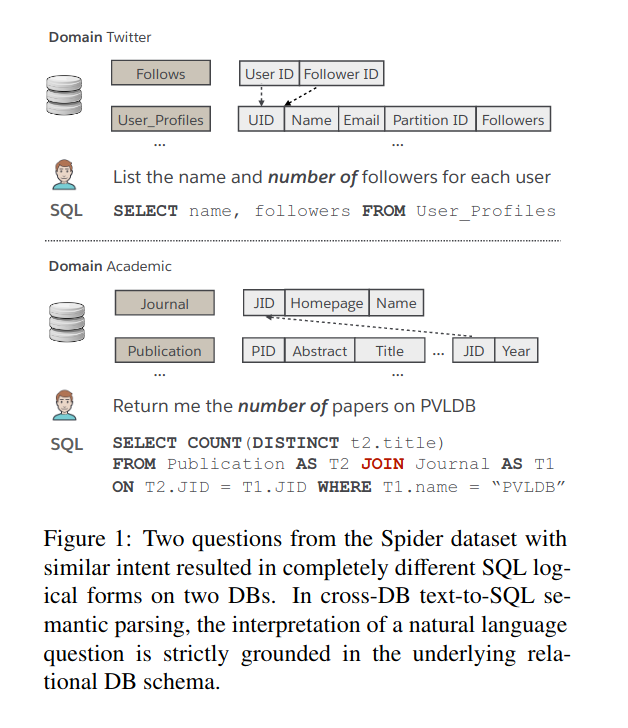
\includegraphics[scale=0.3]{./image/2.png}
\end{center}
\end{figure}  
\section{Literature review}
Text2SQL recently the field has witnessed a re-surge of interest for text-to-SQL semantic parsing, by virtue of newly released large-scale datasets and matured neural network modeling tools. The task uses the model consists of 2 parts: encoder and decoder. Some works like  (Guo et al., 2019; Wang et al.,
2019; Choi et al., 2020; Furrer et al., 2020). Bogin
et al. (2019a,b) encode schemas as graphs and use graph strcutures to guide decoding.  Guo et al. (2019) proposes schema-linking and SemQL, an intermediate SQL representation customized for questions in the Spider dataset which was synthesized via a tree-based decode.. Wang et al. (2019) proposes RAT-SQL, a unified graph encoding mechanism which effec-tively covers relations in the schema graph and its linking with the question. The overall architecture of RAT-SQL is deep, consisting of 8 relational self-attention layers (Shaw et al., 2018) on top of BERT-large.
\begin{figure}[htbp] 
\begin{center}
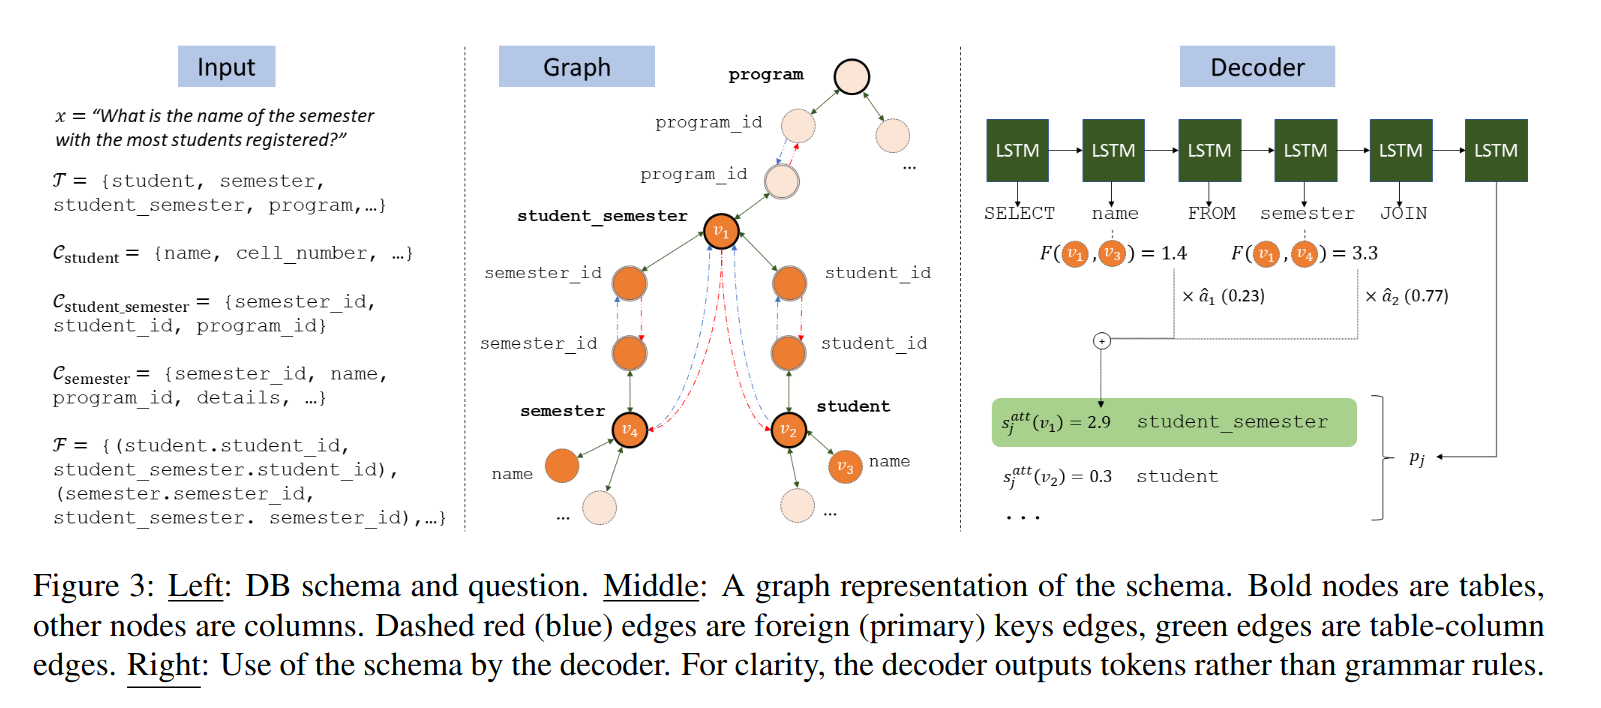
\includegraphics[scale=0.3]{./image/3.png}
\end{center}
\end{figure}
\\ 
Text2SQL can be formulized as seq2seq problem by concatenating natural question and sequential database, then decoder generates sql form. Shaw et al. (2020) shows that the T5 model (Raffel
et al., 2020) with 3 billion parameters achieves the
state-of-the-art performance on Spider. \\
Text2SQL can be enchaned by using DB content. Shaw et al. (2019) shows
that value information is critical to the cross-DB
semantic parsing tasks. \\
BRIDGE is a general framework for jointly representing question, DB schema
and the relevant DB cells. BRIDGE serialized the relational DB schema and uses BERT to model cross-
table dependencies. It uses anchor texts which provide more focused signals that link the text and the DB schema.
\section{Methods}
BRIDGE epresent each table with
its table name followed by its fields. Each table
name is preceded by the special token $[T]$ and each
field name is preceded by $[C]$. The representations
of multiple tables are concatenated to form a se-
rialization of the schema, which is surrounded by
two $[SEP]$ tokens and concatenated to the question.
Finally, following the input format of BERT, the
question is preceded by $[CLS]$ to form the hybrid
question-schema serialization.
\begin{center}
$X = [CLS],Q,[SEP],[T],t_{1},[C],c_{11},...,c_{1|T_1|},[T],t_{2},[C],c_{21},...,c_{N|T_N|},[SEP]$
\end{center}
X is encoded by a Bi-LSTM layer, the question segments output is then passed to another Bi-LSTM. Each table/field is represented
using the slice of output X corresponding to its special
token $[T]/[C]$.\\
Primary keys, foreign keys and data types are also trained by using dense lookup features. These feature then are fused with output X to form final encoding of schema.\\
$\textbf{h}^{t_{i}}_{S} = g([\textbf{h}^{p}_{X};\textbf{0};\textbf{0};\textbf{0}])$ \\
$\textbf{h}^{c_{ij}}_{S} = g([\textbf{h}^{q}_{X};f^{u}_{pri},f^{v}_{for},f^{w}_{type}])$  $=ReLU(\textbf{W}_{g}[\textbf{h}^{q}_{X};f^{u}_{pri},f^{v}_{for},f^{w}_{type}]+\textbf{b}_{g})$\\
$\textbf{h}_{S} = [\textbf{h}^{t_{1}},...,\textbf{h}^{t_{|\tau|}},\textbf{h}^{c_{11}},...,\textbf{h}^{c_{N|T_{N}|}}]$\\\\
Use of anchor text
to link value mentions in the question with the cor-
responding DB fields by performing fuzzy string
match between $Q$ and the picklist of each field in
the DB. The matched field values (anchor texts)
are inserted into the question-schema representa-
tion $X$, succeeding the corresponding field names
and separated by the special token $[V]$. If multiple
values were matched for one field, we concatenate
all of them in matching order. If a ques-
tion mention is matched with values in multiple
fields. We add all matches and let the model learn
to resolve ambiguity. \\ 
The decoder is initiated with the final state of the question encoder. At each step, the decoder performs one of the following actions: generating a token from the vocabulary $V$, copying a token from the question $Q$ or copying a schema component from $S$.\\
\begin{center}
$e_{tj}^{(h)} = \frac{s_{t}W^{(h)}_{U}(h_{j}W^{(h)}_{V})^\top}{\sqrt{n/H}};\space \alpha_{tj}^{(h)}=\underset{j}{softmax}\{e_{tj}^{(h)}\}$\\ 
$z_{t}^{(h)} = \sum^{|Q|+|S|}_{j=1}\alpha_{tj}^{(h)}(h_{j}W^{(h)}_{V});z_{t}=[z_{t}^{(1)},...,z_{t}^{(H)}]$\\
$p^{t}_{gen}=sigmoid(s_{t}W^{s}_{gen}+z_{t}W^{z}_{gen}+b_{gen})$\\
$p^{t}_{out} = p^{t}_{gen}P_{\mathcal{V}}(y_{t})+(1-p^{t}_{gen})\sum_{j: \overset{\sim}{X}_{j}=y_{t}}\alpha_{tj}^{(H)})$
\end{center}
\begin{figure}[htbp] 
\begin{center}
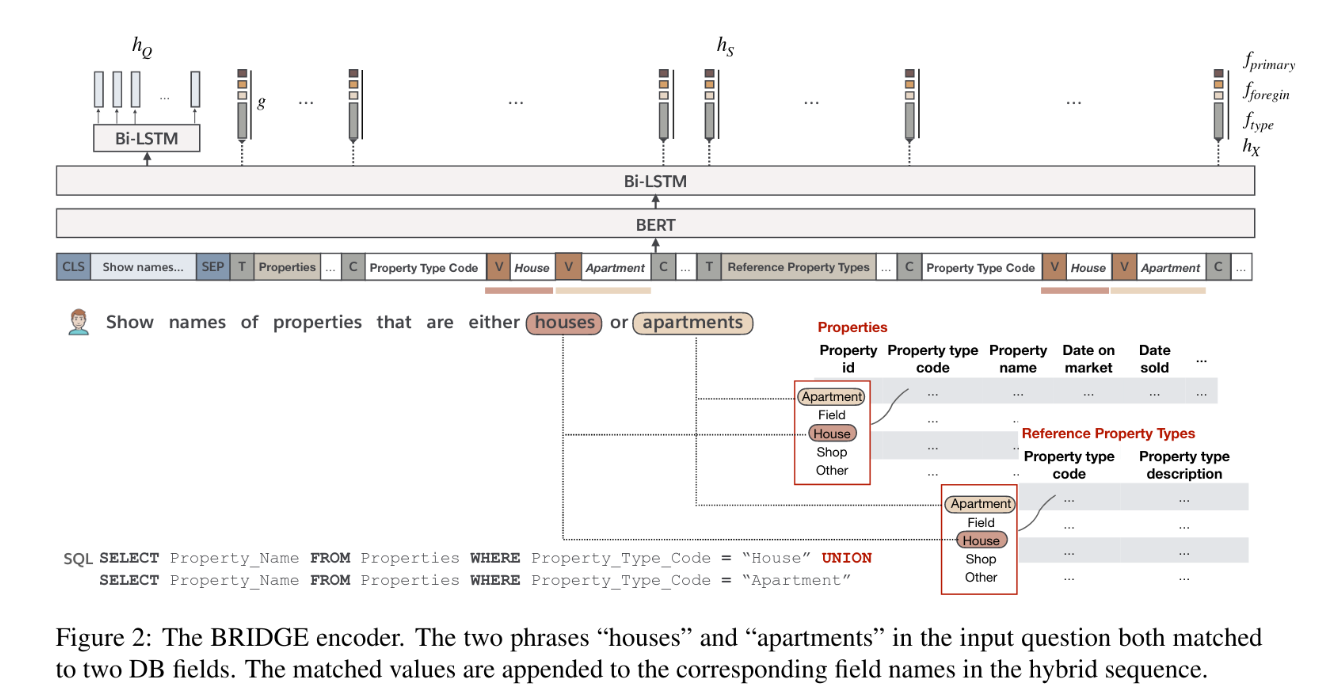
\includegraphics[scale=0.3]{./image/1.png}
\end{center}
\end{figure}
The fact that the DB fields ap-
peared in each SQL clause must only come from
the tables in the FROM clause. \\
\textbf{Lemma 1} Let $Y_{exec}$ be a SQL query with clauses
arranged in execution order, then any table field in
$Y_{exec}$ must appear after the table.\\
As a result, we adopt a binary attention mask $\xi$\\
$\overset{\sim}{\alpha}_{t}^{(H)}=\alpha_{t}^{(H)} . \xi$\\
which initially has entries corresponding to all
fields set to 0 Once a table $t_{i}$ is decoded, 
all entries in $\xi$ corresponding to that table to 1, allows the decoder to only search in the space
specified by the condition in Lemma 1 with little
overhead in decoding speed.
\section{References}
1. https://github.com/salesforce/TabularSemanticParsing \\
2. arXiv:1706.03762 \\
3. Xi Victoria Lin, Richard Socher, and Caiming Xiong. 2020. Bridging Textual and Tabular Data for Cross-Domain Text-to-SQL Semantic Parsing. In Findings of the Association for Computational Linguistics: EMNLP 2020, pages 4870–4888, Online. Association for Computational Linguistics.\\
4. Bailin Wang, Richard Shin, Xiaodong Liu, Oleksandr Polozov, and Matthew Richardson. 2020. RAT-SQL: Relation-Aware Schema Encoding and Linking for Text-to-SQL Parsers. In Proceedings of the 58th Annual Meeting of the Association for Computational Linguistics, pages 7567–7578, Online. Association for Computational Linguistics.\\
5. https://www.microsoft.com/en-us/research/uploads/prod/2018/07/Execution-Guided-Neural-Program-Decoding.pdf
\end{document}